\chapter{Concept \label{chap:concept}}

%Big picture
%General ideas how to solve goals
%Present equal concepts with theoretical pro's and cons
%What are the general ideas that we try to solve the problem with?

In order to deal with the continuous information stream a robot experiences when it interacts with an unknown environment, a robot needs an architecture.
This architecture needs to organize the incoming data and determine what should be learned from these experiences. Furthermore, the architecture can combine different components in order to make the best use of what it has already learned. 
This chapter presents the two concepts that were developed in order to learn about simple object interactions. These two concepts differentiate mainly in the way they represent the interactions that they learn about. The first concept, further described in section \ref{sec:pairInt}, uses pairwise interactions to represent the objects in the environment. In the alternative approach, described in section \ref{sec:gate}, the objects are represented individually. Additionally, a gating function is introduced to distinguish when one object actually influences another. 
A special inverse model is proposed in section \ref{sec:invModel} that is tailored to the continuous interaction with the environment. 
Before going into the description of both concepts and the inverse model, section \ref{sec:problem} summarizes the actual problem these concepts need to solve. 

\section{Problem specification \label{sec:problem}}

As stated in the introduction, the goal of this thesis is to provide possible models that incrementally learn simple pushing interactions between physical objects. 
More specifically, the models need to learn two tasks:

1) Given some known action primitive that controls the robots actuator, the models need to learn to predict the next states of all objects in the environment (\textit{forward model}). 
While these action primitives are determined beforehand, the models do not necessarily know the effects of the primitives. In this case, the models need to not only learn about the pushing interactions, but also about the consequences of their own actions.

2) The robot is supposed to be able to reach some specified target configuration (\textit{inverse model}). Any object in the environment, not just the actuator, can be specified which means that the models must learn how they can influence the objects through their actuator. The target configurations will rarely be reachable within a single action primitive but the inverse model should still provide actions that reduce the distance to the target configuration. 
Since the actuator can only influence another object by pushing it, the actuator might be required to circle around an object in order to be able to move it towards the desired configuration.

A sequence of action primitives that would reach the target after their execution is not requested. This is because the models are expected to react to changes in the environment directly. Furthermore, if such a sequence is required, for example in order to make higher level plans, they can be created using the described forward and inverse models.

Both of these tasks need to be learned incrementally without prior training. This requires the models to be tightly coupled to the environment. An overview about the models interaction with the environment can be seen in figure \ref{fig:overview}. The models are updated each time feedback from the environment is received, improving the quality of following predictions.

\begin{figure}
	\centering
	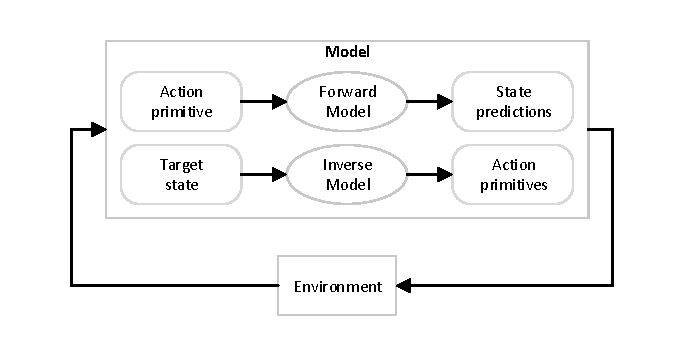
\includegraphics{Overview.pdf}
	\caption{Overview of the problem. The desired models need to include a forward model in order to make predictions given the current environment state and a certain action primitive. When given a target state an inverse model provides suitable action primitives to reach the desired state.}
	\label{fig:overview}
\end{figure}

\section{Modeling pairwise interactions \label{sec:pairInt}}

The first approach that is proposed here tries to find distinct subspaces in the \textit{interaction space} between two objects. In this context, the pairwise interaction space represents the space of all interactions between two objects. This includes their relative placement and movement to each other, as well as their influence, for example by pushing, on each other. Instead of modeling and learning forward and inverse models for each object separately, only the pairwise interaction space between two objects is considered. 

For every object pair an \textit{interaction state} is considered. This interaction state represents one object's state relative to the other object's state. This includes for example transforming each object's position and orientation to the local coordinate system of the reference object. %For the realization, described in section \ref{sec:pairRealization}, he actuator is not used as reference.
The predicted object states are extracted from the predicted interaction states. The way these interaction states are computed from the object states and how the object states can be extracted from the predicted interaction states, need to be provided to the model beforehand. Considering the robotic context, this means that the way the robot's sensor inputs are combined into features need to be predetermined.

At each update step the current interaction states for all object pairs are computed from the information provided by the environment. The previous state, the performed action and the resulting state are collected and stored as an \textit{episode} $e$. The general idea is to store these episodes as past knowledge, similar to the approach in case based reasoning \cite{cbr}. When predicting, these episodes can be searched for the most similar one. The similarity can be determined by comparing the previous state of each episode to the given interaction state and the used action to the current action:

\begin{equation}
e^{best} = \argmin_{e^i \in E} ||e^i_{preState}-curState, e^i_{action}-curAction||_{ep}
\label{eq:bestEpisode}
\end{equation}


$e^i$ represents the i's episode that has been stored yet. $e^i_{preState}$ means only the previous interaction state of the episode, while $e^i_{action}$ represents the used action in that episode.
The norm $||a,b||_{ep}$ is used to allow different weighting of the features from the previous state and the action. For planning, the action difference can be replaced by the difference between the resulting state of each episode and the desired target state.

Once the most similar episode has been found, the desired information can be extracted from it. For prediction, this corresponds to the resulting state in the episode, whereas it corresponds to the action for the inverse case. The formula above represents a nearest neighbor search on all episodes. Although such an approach can work, it quickly becomes infeasible when the number of stored episode keeps growing. Since the nearest neighbor search scales linearly with the number of stored examples it is unsuitable for lifelong learning. 
Furthermore, the simple nearest neighbor approach does not offer good generalization since it does not interpolate between similar episodes. 

As mentioned at the beginning of this chapter, the idea of this concept is to split the interaction space into subspaces and train local models for each of these subspaces. This concept and it's implementation will often be referred to as \textit{interaction state concept/model} for the remainder of this thesis accordingly.
An overview of the proposed architecture can be seen in figure \ref{fig:PairOverview}.
All episodes corresponding to the same subspace are collected in \textit{\glspl{ac}}. Each collection can train its own local forward and inverse model which is explained in section \ref{sec:ACs}.
An \textit{\gls{acs}} is needed in order to choose the most appropriate \gls{ac} in a given situation. 


\begin{figure}
	\centering
	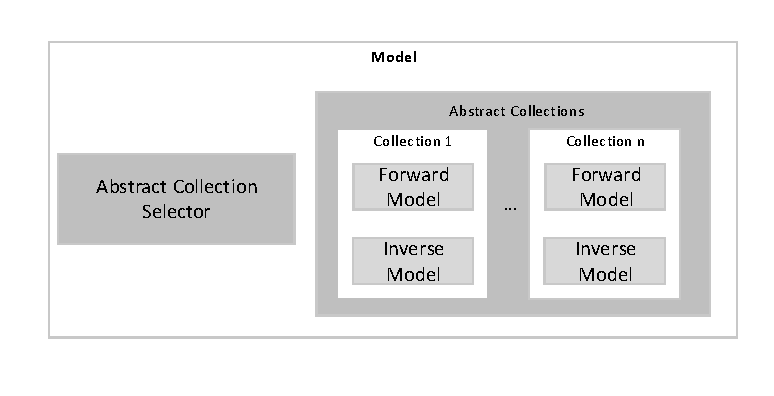
\includegraphics{PairwiseOverview.pdf}
	\caption{Overview of the interaction state model. The different \acrlongpl{ac} contain forward and inverse models of distinct subspaces of the interaction space. The selector is needed in order to select the appropriate local model for prediction.}
	\label{fig:PairOverview}
\end{figure}

\subsection{Abstract Collection \label{sec:ACs}}

The interaction space can be split in a multitude of subspaces. Ideally, one would want to split the space in subspaces with some semantic meaning, for example into \textit{no interaction}, \textit{turning} and \textit{pushing}. In this example, the no interaction subspace would correspond to the episodes where the actuator moves without influencing another object. Turning would correspond to an interaction where mainly the orientation of an object changes through the interaction. Lastly, the position of an object changes mainly in the pushing subspace. However, in order to separate the episodes like that, accurate labels are required. Such a classification is infeasible without prior domain knowledge. 
Instead of relying on domain knowledge, this approach uses the information available to the robot from the environment: The changing features within an episode.

In order to split the interaction space into subspaces, episodes that correspond to the same local group are clustered together.
The clustering of episodes suggested here is based on the set of features that changed between the previous state and the resulting state after performing an action. The set $S$ of features that changed is defined as follows 
\begin{equation}
S = \{f | f \in F ~ \wedge ~ ||Pre(f)-Post(f)|| > \epsilon_{Noise}\}
\label{eq:difSet}
\end{equation}
where $F$ denotes the set of all features. $Pre(f)$ and $Post(f)$ denote the value of 
feature $f$ in the initial and resulting state of the episode respectively. $\epsilon_{Noise}$ is a threshold to cancel out potential noise of the environment and should be set according to the accuracy of the used sensors. Ideally, one would like to have feature specific thresholds since the possible range of the features might vary. However, this would require the model to have additional information about each feature.

Each different set is represented by its own \acrlong{ac}. The 
idea is that, while not necessarily holding semantic meaning directly, these collections correspond to different interaction scenarios. Depending on the features used, some \glspl{ac} might even be interpreted semantically.
Consider an exemplary interaction state with two features. The first feature represents the closest distance between the two objects in the interaction state. The second feature represents the angular direction of the second object with respect to the local coordinate system of the reference object. While the model itself has no knowledge about what each feature represents, a maximum of four \glspl{ac} can be created: No feature changes, either one of the two features changes and both change at the same time. In this example the \gls{ac} containing only the distance feature represents all interactions where one object moves straight towards or away from the other object. The set where nothing changes would signal a pushing interaction, considering a movement action was performed. While not all created \glspl{ac} can be interpreted semantically, the model can create these separations without any knowledge about what is represented by the features.

Since each distinct interaction scenario results in a different set of changing features, the interaction space is split into subspaces by these collections. The resulting collections create an abstract representation for each of these interaction scenarios. 

These collections can then train their respective local forward and inverse models based on the episodes associated with them. Any suitable regression method can be used for these local models. The above mentioned nearest neighbor structure that works directly on the recorded episodes is just one simple example. Since the collections are independent of each other, different collections can even use different methods if desired. Furthermore, local optimizations such as feature selection could be performed in each collection. 

\subsection{Object state prediction with the Abstract Collection Selector \label{sec:pairPrediction}}

Predicting object states within this concept requires several steps since only interaction states are modeled explicitly. The general idea of the information flow when predicting one interaction state is visualized in figure \ref{fig:PairPrediction}. The model expects an interaction state that has been computed from the objects' information provided by the environment. This interaction state is used together with the given action primitive as input for the \acrfull{acs}. The selector needs to estimate which \gls{ac} is most likely responsible for the next interaction. In order to make this estimation, any suitable classifier, e.g. a decision tree \cite{decisionTree}, is trained on all input-collection pairs the model experienced so far. 
The total number of collections is limited to the size of the superset of $F$, although in practice, not all possibilities are likely. Furthermore, collections with less than $\epsilon_{min}$ episodes could be ignored. This threshold can be used to reduce the number of outliers when training the classifier. 

After the most likely \gls{ac} has been selected, its forward model can be consulted for the prediction. The local model is queried using the interaction state together with the given action primitive as input. The output of the local model is the predicted interaction state. 
More precisely, the local model predicts how the current interaction state changes within the features defined by its set of changing features $S$.
These predicted changes are then added to corresponding features dimensions of the given interaction state that this \gls{ac} is responsible for.
The predictions of the actual object states need to be extracted from this interaction state. The extraction depends on the actual features used and needs to be provided by the user just like the structure of the interaction state itself.

\begin{figure}
	\centering
	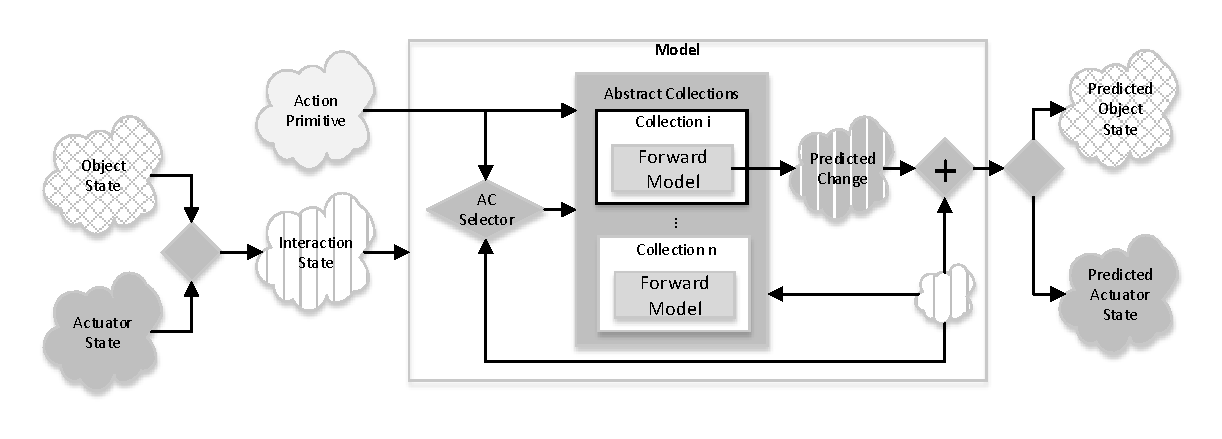
\includegraphics[width=\textwidth]{PairwisePrediction2.pdf}
	\caption{Concept of prediction in the pairwise interaction space with \acrfullpl{ac}. First the interaction state is computed. This state is then fed to the model together with the chosen action primitive. The \acrlong{acs} (AC Selector) uses those to select the responsible \gls{ac}. The collection then uses its forward model to predict the changes in the interaction state. These changes are added to the given interaction state in order to compute the resulting prediction. Finally, the actual predicted object states are extracted from this interaction state.} 
	\label{fig:PairPrediction}
\end{figure}

\subsection{From target state to action primitive \label{sec:pairPlanning}}

In order to get a suitable action primitive given a target configuration several steps are required as visualized in figure \ref{fig:PairPlanning}. 
First the difference state between the current situation and the target configuration is computed. Similar to the computation within the episodes above, a difference set $S$ can be computed from this difference state. Afterwards, the \gls{ac} that corresponds to the same set of features is selected. In the case that this collection is not yet known, the most similar collection is chosen instead. In this context, the most similar \gls{ac} is the one that covers most of the changed features in the computed difference set. If multiple alternatives exist, the \gls{ac} responsible for the changes in the most features is chosen. This is because the inverse model has more degrees of freedom to reach the target in that case.

The selected \gls{ac} queries its own inverse model for preconditions that produce a change in the direction of the desired target configuration. 
Only returning the corresponding action primitive is not sufficient, since it might not be possible to move an object directly in the desired direction due to the current position of the actuator.

The preconditions need to be checked against the current configuration of the target object and the actuator. If these preconditions are mostly fulfilled an action primitive can be extracted, otherwise an intermediate target needs to be determined. This intermediate target represents a configuration for the actuator where the preconditions are met. The actuator might be required to circle around the object in order to reach the intermediate target without influencing the object in a negative way.


\begin{figure}
	\centering
	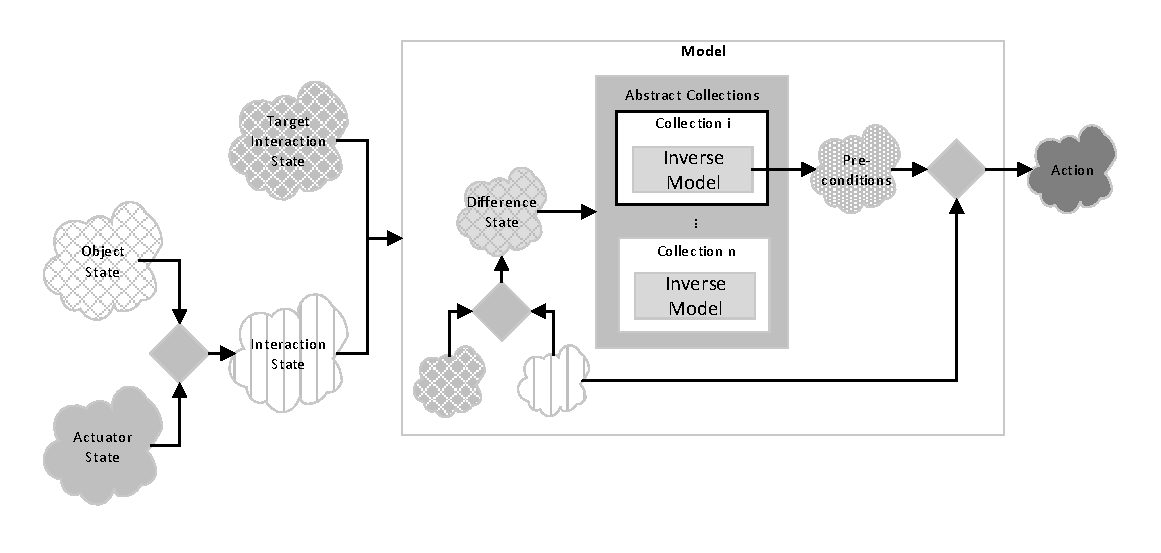
\includegraphics[width=\textwidth]{PairwisePlanning.pdf}
	\caption{Concept of computing suitable action primitives in order to reach a given target configuration within the interaction state concept. The suitable \gls{ac} is determined by the Difference State. An action primitive is computed from the preconditions returned by the inverse model.} 
	\label{fig:PairPlanning}
\end{figure}


\subsection{Theoretical discussion \label{sec:interactionTheory}}
The two core ideas of this concept are the use of a pairwise representation and splitting the interaction space. The splitting is done in order to allow the training of simpler local regression models. Furthermore, using local models avoids having to compare to all previously seen training examples. However, this does require the \acrlong{acs} in order to first select the correct local model.
Using a global regression model, for example for the inverse model, is obviously possible as well, especially if the used model does not suffer from the complexity of the used interaction state and the continuous training. Global models have the benefit of not having to determine the responsible \acrlong{ac}.

Using pairwise interaction states in order to represent the interactions between objects is often used in robotics, for example in \cite{moldovan2012learning,pairwise2}. 
Its advantage is that it represents both objects involved in an interaction at the same time. This means that only one regression model needs to be trained in order to make predictions about both objects. In theory this should also make it less likely that impossible configurations are predicted such as solid objects being inside of each other. Furthermore, such an interaction state can contain all the necessary information about the objects in one representation. 

The downside of this approach is that the actual object states need to be inferred from these interaction states. When using only differential features to construct the pairwise interaction state, this will only involve simple coordinate transformations. Some other object attributes might not be as easily transformable though. Furthermore, in order to contain all the necessary information about both objects, these interaction states can become high dimensional. All computations from object to interaction states and vise versa need to be performed outside this proposed model and need to be predefined.

Although the coupling of the two objects can have its advantages as stated above, the dependence between the objects can also be a problem when predicting. Any erroneous prediction will immediately affect two objects. 
Furthermore, when one of the two objects is represented relative to the coordinate frame of the other object, all predictions are also made with regard to the reference object's coordinate frame. 
In case the state of the reference object is not accurate, for example because of a sensor malfunction, the predictions for both objects will be influenced by this error.
This can easily be imagined when considering errors in the reference object's position. Since the second object's position needs to be computed based on the reference object's position, the error will immediately be reflected in the predictions for both objects.

An even bigger disadvantage is the fact that this approach cannot easily be extended to multiple objects. In environments with at least two objects and an actuator at least three pairwise interaction states are necessary: One for the first object and the actuator, one for the second object and the actuator and at least one for both objects. 
While one can argue for and against using the actuator as the reference object for the general case, depending on the actual scenario, this decision is not trivial between two objects. 
Even if one finds suitable reference objects, there is still a problem with the extraction of the actual object states after prediction. All objects are part of at least two interaction states in this situation. Therefore, at least two extracted predictions exist for all objects in the environment. Unfortunately, these predictions are likely to be different from another. It is therefore required to compute a final prediction for each object which is not trivial in the general case. Furthermore, the presented concept does not even know about object states, meaning that the final computation would need to be performed outside of the concept.
It is also unclear if an \gls{ac} should only be responsible for the interaction subspace between two specific objects or if its local model should represent the subspace for all object pairs. In most cases, training individual \glspl{ac} for each object pair is likely to be more successful because similar actions will result in different interactions for different interacting objects.

%Regardless of the used representation, the proposed concept might have further issues:
Regarding the \acrlongpl{ac}: 
Unfortunately, no guarantees can be given about how well the interaction space is split. Depending on the used features, as well as the actual interaction scenarios that are encountered, some abstract collections might cover most of the interaction space. 


\section{Object space with gating function \label{sec:gate}}

The intuitive alternative to modeling the interaction space, is to model each object and perform predictions for each object separately. 
The general components of this architecture are visualized in figure \ref{fig:GateOverview}.

\begin{figure}[h]
	\centering
	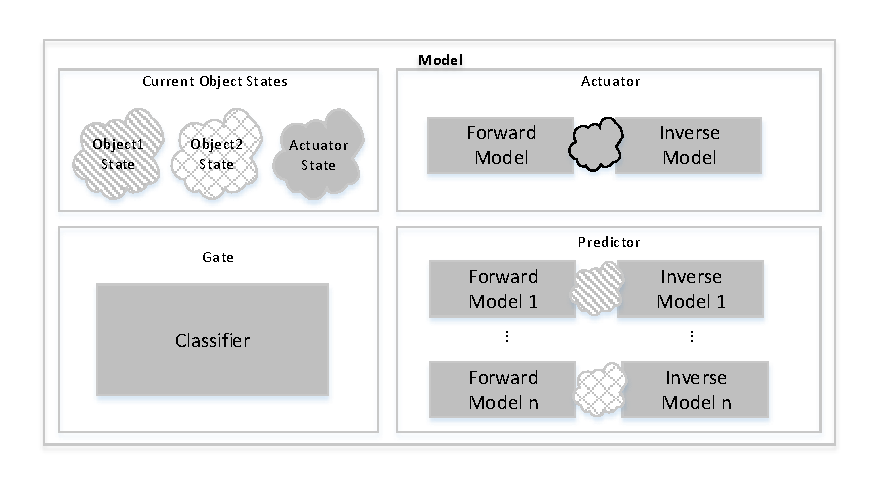
\includegraphics{GateOverview.pdf}
	\caption{Overview of the concept using object state with a gating function. The actuator is a special object, that can be influenced directly. It's forward and inverse model might even be provided if known. For the other objects/object groups, the Predictor learns these models. The gating function (Gate) learns a classifier to distinguish interactions between objects from situations where only the actuator changes.} 
	\label{fig:GateOverview}
\end{figure}

The idea is to train local forward and inverse models for each object, or object group in the \textit{Predictor}. 
Instead of distinguishing between different interaction scenarios as in the previous concept, objects that behave differently are distinguished. 
An object group can be considered a collection of objects that are similar in the way they behave during interactions. Therefore they can be represented by a single local model. One example would be two identically shaped block objects that only have different colors. In order to detect if two objects should be grouped together or not, one can start with training separate local models and compare their outputs. If two models appear to be similar, they can be merged together. Ideally, a similarity measure for objects is provided. Following the assumption that similar objects should behave similarly, such a measure would allow immediate grouping of objects.

Apart from the difference in representation, the other big difference in the two concepts is the introduction of the gating function (\textit{Gate} in the figure). The gating function is used to split the interaction space in two big subspaces. The first subspace represents all scenarios where at most the actuator is moving due to some action primitive but no other object is influenced by the actuator. In the given context, this means that no actual pushing interactions are taking place.  Consequently, the other subspace contains all the scenarios where an object is influenced. When making predictions for the first subspace, it is sufficient to make predictions about the next state of the actuator. No knowledge about the behavior of the objects is required which also means that the local models do not need to be trained for these scenarios. The local object models only need to be trained on the scenarios where an object's state actually changes. 
This makes the local subspaces each model needs to learn already simpler then the interaction space learned in the previous concept. Therefore, multiple models for each object are not required.

In order to allow the local models to only train on this restricted subspace, this concept makes an additional assumption about the environment: 
This idea assumes that object states do not change without any interaction. The only exception is the \textit{Actuator}. Here, the actuator is treated as a special kind of object with its own forward and inverse model. These models can be provided beforehand or learned online.  

The current state of each object, including the actuator, is always updated when new information is received from the environment. At each update the gating function and if required the actuator's local models are trained. On top of that, the local models responsible for any objects whose states have changed with the last update, are trained as well. 

Due to the significance of the gating function, this concept and its implementation will often be referred to as \textit{gating concept/model} in the remainder of this thesis.



\subsection{Object state prediction \label{sec:gatePrediction}}

Because of the assumption that objects other than the actuator cannot change without any interaction, the way prediction is performed differs between the different object types. The actuator simply queries its own forward model with the selected action primitive as input in order to predict the next actuator state. 
The general process for predicting the next state of other objects is visualized in figure \ref{fig:GatePrediction}.

\begin{figure}[h]
	\centering
	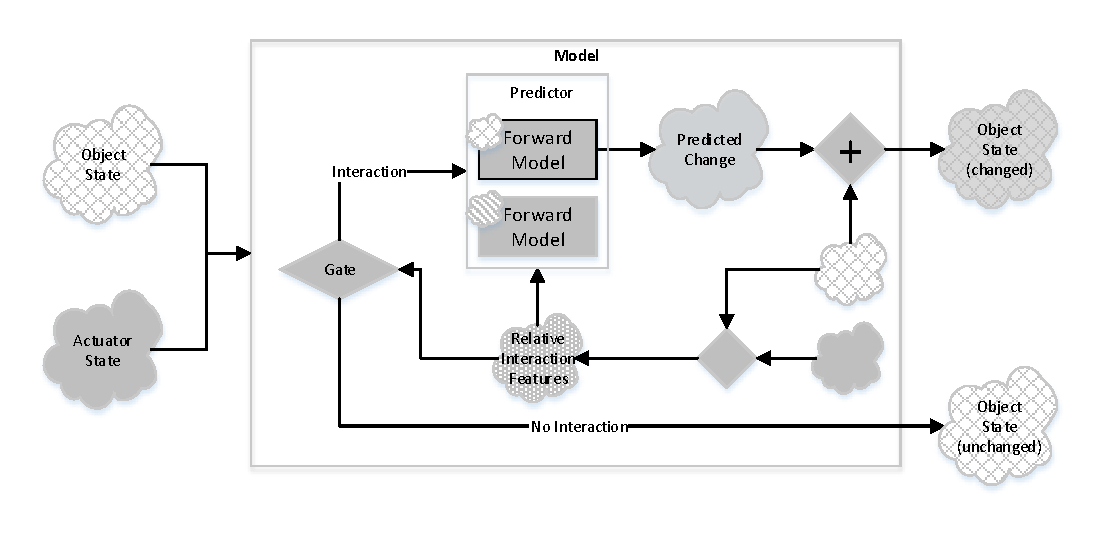
\includegraphics[width=\textwidth]{GatePrediction.pdf}
	\caption{Visualization of the prediction process for non actuator objects in the gating concept. Using the predicted actuator state, relative interaction features are computed. These are used by the gating function to determine if an interaction takes place or not. The responsible local forward model is used to predict 
	changes in the object's state if an interaction is expected. From these changes the actual state prediction is computed.} 
	\label{fig:GatePrediction}
\end{figure}

First the next actuator state is predicted as mentioned above using the selected action primitive.
This predicted state is then used together with the current state of the object that is to be predicted to compute \textit{Relative Interaction Features}. These relative features are similar to the pairwise interaction state that was explained in the previous concept. However, since it is not necessary to extract the entire object state for both objects from these relative features, the dimensionality can be a lot lower than before or additional higher level features can be used. In fact, depending on the scenario, it may be sufficient to only represent the actuator in the local coordinate frame of the object. 
The gating function then uses these features to determine if the object will be influenced by the new actuator state. If the gating function predicts no interaction between the object and the actuator, the current object state is returned. 
On the other hand, if an interaction is predicted, the \textit{Predictor} uses the local forward model responsible for the current object. 
The local model predicts the changes in the object states instead of the final states. In order to get the actual predicted object state, these changes are added to the current object state.

When more than one object other than the actuator is present, the same process can be repeated. 
In order to predict interactions between two non actuator objects, a prediction chain is performed. First the actuator is predicted as described above. Afterwards, the objects that are directly influenced by the actuator are predicted. 
The predictions of these objects can then in turn be used as new \enquote{actuators} for interactions between them and other objects. However, additional problems arise as explained in section \ref{sec:gateTheoDisc} below.

\subsection{From target object state to action primitive \label{sec:gatePlanning}}

Similar to prediction, computing a suitable action primitive is performed differently depending on what kind of object is supposed to reach a given target configuration. In the case that the target object is the actuator, its inverse model is queried for an action primitive with the target configuration as input. 

The more interesting process of moving towards a target configuration for a non actuator object is visualized in figure \ref{fig:GatePlanning}.

\begin{figure}
	\centering
	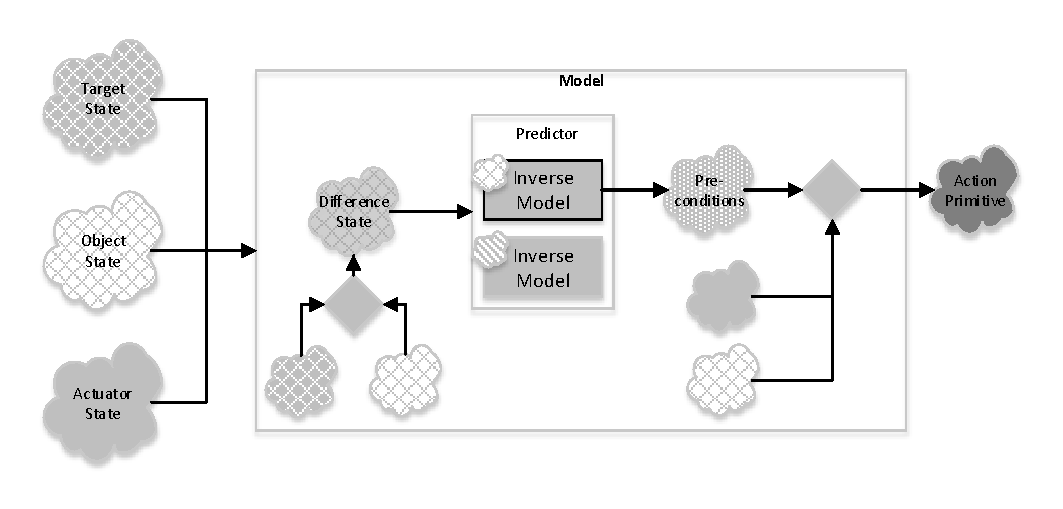
\includegraphics[width=\textwidth]{GatePlanning.pdf}
	\caption{Visualization of the process of computing action primitives to move non actuator objects towards a target configuration in the gating concept. Using the Difference State as input, the local inverse model responsible for the target object are queried for Preconditions. The resulting action primitive is computed from these preconditions.}
	\label{fig:GatePlanning}
\end{figure}
	
First the current difference state is computed from the given target configuration and the current object state. This difference state is then used to query the inverse model responsible for the target object. Since only the actuator can be influenced by action primitives directly, these local inverse models do not directly return action primitives. Instead they return preconditions in the form of the relative interaction features. These features represent a situation where the object state changes in the direction of the target configuration. 
	
The current actuator state is then compared to these preconditions. If the actuator is already in a configuration where it meets these preconditions, an action primitive is derived from the local features. This requires that the local features contain information that can be used to compute an action primitive.
However, in most situations the actuator configuration will not meet the preconditions. The given preconditions will often require the actuator to be in a different position relative to the object that is to be moved. In these cases the suitable position for the actuator is used as an intermediate target. 

Considering the current object's position, an action is calculated to move the actuator towards the intermediate target. It might be necessary to perform a circling movement around the object. Moving the actuator directly towards the intermediate target position might result in moving the object in a more unfavorable position and is therefore avoided. Since these steps are performed at every timestep, the model can quickly adapt itself to changes in the environment.
	
\subsection{Theoretical discussion \label{sec:gateTheoDisc}}

Representing each object by itself has the advantage, that no transformations outside of the concept are required. Instead all objects are represented for themselves within the model. 
Consequently, any noise in any object does not directly influence another object's state directly. Noisy data in one object might still influence the prediction of another object, for example if the noise leads to an erroneous classification by the gating function. However, the effect is not as unavoidable as in the pairwise interaction concept.

The big disadvantage of this approach is that impossible configurations can be predicted more easily. This can happen due to an inaccurate prediction made by either the actuator's or the object's forward model.
An impossible configuration is even bound to be predicted when the gating function misclassifies that no interaction takes place when it should. In this case the actuator is predicted to move into the other object.

Extending this concept to multiple objects is easier in theory since each object can be considered separately. However, training the gating functions with multiple objects is difficult. When one object's state changes during an update from the environment, the model needs to determine which other object caused this change in order to train the gating function on the correct relative interaction features. Depending on the situation, this causal determination can be very difficult and hardly be done without additional prior knowledge. 

Apart from the representation, this concept requires an additional assumption about the scenario compared to the interaction state concept. The assumption that object states can only change through interactions with an actuator also means that an object does not continue sliding after it has been pushed. This restricts the possible weights of the objects and speeds of the actuator.
A possible solution that was not pursuit within this thesis would be to predict the forces that operate on each object instead of the resulting object state. Using the forces, each object could train its own forward model which predicts the next state based on these forces. This however requires the robot to be able to detect or estimate these forces. Furthermore, predicting forces is often more complex then predicting static attributes such as position or orientation.


\section{The Averaging Inverse Model\label{sec:invModel}}

In order to compute suitable action primitives given a target configuration, both concepts require inverse models.
Directly searching in the forward regression model for the inverse has two disadvantages in the given scenario: 

\begin{enumerate}
\item The difference state that is computed can have features orders of magnitude greater than any change the local models have been trained with. In fact any target configuration, that requires multiple timesteps to reach, is already outside the range of the changes the forward models can have seen. 
The inverse model would need to extrapolate into unknown regions in these cases.
\item The features in the target state are not necessarily normalized. Therefore, the model does not necessarily know if a reduction of the difference in one feature is better than in another. This especially becomes a problem once only actions can be found that decrease the difference in one feature dimension at the cost of an increase in another feature dimension. Consider the example where a target position and orientation is given for an object. There might be situations where the object needs to be turned away from the target orientation in order to reduce the distance to the target position. In this case the orientation would need to be more or less ignored when using the inverse model to search for an action.
\end{enumerate}
%1) The difference state that is computed can have features orders of magnitude greater than any change the local models have been trained with. In fact any target configuration, that requires multiple timesteps to reach, is already outside the range of the changes the forward models can have seen. 
%The inverse model would need to extrapolate into unknown regions in these cases. \\
%2) The features in the target state are not necessarily normalized. Therefore, the model does not necessarily know if a reduction of the difference in one feature is better than in another. This especially becomes a problem once only actions can be found that decrease the difference in one feature dimension at the cost of an increase in another feature dimension. Consider the example where a target position and orientation is given for an object. There might be situations where the object needs to be turned away from the target orientation in order to reduce the distance to the target position. In this case the orientation would need to be more or less ignored when using the inverse model to search for an action.

Furthermore, the output of the inverse model does not need to be as precise as the predictions of the forward model. This is mainly due to the fact that the inverse model is used to reach a target configuration interactively. In the context of this thesis, there is no need to provide a sequence of precise action primitives that will then be executed blindly. Instead, as highlighted in figure \ref{fig:overview}, the model is tightly coupled with the environment. This means that the model is constantly updated and can adapt to changing situations. It is therefore sufficient for the inverse model to provide the means to make a step in the direction of the target configuration. In the context of the two concepts presented here, the means are not directly action primitives but rather preconditions that need to be fulfilled in order to be able to influence an object in a certain way.

In order to avoid the mentioned problems, a special inverse model is proposed that is trained separately from the forward model:
The model is called \textit{\gls{tiim}} due to its nature of computing average preconditions for certain effects.
%It is called \textit{\gls{tiim}} because, unlike a forward model, it does not focus on the actual quantity of the feature changes within one timestep. 
Unlike a forward model, it does not focus on the actual quantity of the feature changes within one timestep. 
Instead, the inverse model focuses mainly on the direction, or the sign, of the changes. Furthermore, in order to avoid the problem of weighting feature importance, each feature dimension is considered separately. 

For each feature dimension, the model collects all the preconditions that result in a positive and negative change in that dimension separately. Here preconditions means a representation of the situation in which the change occurred.  
An example of this grouping is visualized in figure \ref{fig:InverseModel}. 

\begin{figure}
	\centering
	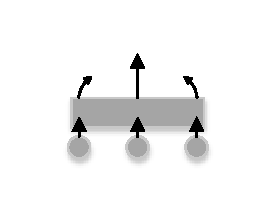
\includegraphics{InverseModel2.pdf}
	\caption{Visualization of the precondition grouping in the proposed \acrlong{tiim}. The arrows above the block symbolize the change in the object's state corresponding to the actuator situations below the block. All three pushing scenarios indicated by the three spheres, will be grouped together since they all result in the same upward positional change.}
	\label{fig:InverseModel}
\end{figure}

The figure shows three different scenarios or preconditions in the form of the three spheres that represent the actuator. In the forward model each precondition is tightly coupled to its resulting change. In this example the left situation results in the small positional change upwards and a negative change in orientation. The same tight coupling is present with the other two situations. In the inverse model proposed here, all three situations are grouped together in one \textit{prototype} responsible for a positional change upwards. Other prototypes exist for the two directions of change in orientation. This way one situation will be included in multiple prototypes if it has caused multiple features to change.

Each prototype creates a weighted average\footnote{Depending on the used features, a simple average does not work. See the implementation details in section \ref{sec:invModelRealization} for details.} of the preconditions for its feature dimension and sign. The preconditions are weighted by their contribution towards the feature dimension. In the example above, the preconditions for the middle scenario receive the strongest weight since they are responsible for the biggest change in position. 

When the inverse model is queried given some difference vector to the target configuration a greedy strategy is used to reduce the feature dimension with the biggest difference first. 
The feature dimension along with the sign of this dimension in the difference vector determine the responsible prototype. The average computed by that prototype can then be used as preconditions that will reduce the distance to the target configuration.



	
